\documentclass[../main.tex]{subfiles}

\graphicspath{{ima/clase14}{ima}}

% Aquí empieza el documento{{{
\begin{document}
\chapter{Hollo-polluelo}%

\thispagestyle{fancy}

\section{Principio del palomar, casillero, Hoyo-polluelo}%
\label{sec:Principio del palomar, casillero, Hoyo-polluelo}

\textbf{Si hay más polluelos que hoyos entonces algunos polluelos duermen juntos.}
\[
	f:[n]\longrightarrow[m]\quad \text{si }n > m
\]
y $f$ es total entonces $f$ no es $\overbrace{|:|}^{\substack{
\text{Total}\\
\text{inyectiva}\\
\text{sobreyectiva}
} }$ (No es inyectiva)


\begin{figure}[H]
	\begin{center}
		\begin{tikzpicture}[scale=1, transform shape]
			\draw (-2,1) ellipse (1 and 2);
			\draw (-2,-1.5) node {Polluelos};

			\draw (2,1) ellipse (1 and 2);
			\draw (2,-1.5) node {Hoyos};

			\draw (-2.25,2) rectangle +(0.5,0.5);
			\draw (-2.25,1) rectangle +(0.5,0.5);
			\draw (-2.25,0) rectangle +(0.5,0.5);

			\draw (2,1.75) ellipse (0.5 and 0.5);
			\draw (2,0.25) ellipse (0.5 and 0.5);

			\draw [arch, dashed, ultra thick, ->] (-2,2.25) -- (2,1.75);
			\draw [arch, dashed, ultra thick, ->] (-2,1.25) -- (2,0.25);
			\draw [arch, dashed, ultra thick, ->] (-2,0.25) -- (2,1.75);
		\end{tikzpicture}
	\end{center}
\end{figure}
Algún valor del rango recibe al menos dos flechas.

\section{Menús}%
\label{sec:Menús}

\begin{enumerate}
	\item Si hay más \textcolor{red}{\bfseries Días del año} que
		\textcolor{red}{\bfseries platos},
		entonces se repiten algunos
		\textcolor{red}{\bfseries platos}.
	\item $36$ personas ¿Al menos cuántos comparten el mismo mes de cumpleaños?

		\begin{figure}[H]
			\begin{center}
				\begin{tikzpicture}[scale=1, transform shape]
					\foreach \y in {1, ..., 10}
					{
						\draw (-2,\y) node {\y};

						\draw (2,\y+0.5) rectangle +(2,-1);
						\draw (4.5,\y) node {\y};
					}
					\foreach \y in {11, ..., 12}
					{
						\draw (2,\y+0.5) rectangle +(2,-1);
						\draw (4.5,\y) node {\y};
					}
					\foreach \y in {1, ..., 3}
					{
						\draw [arch, dashed, ultra thick, ->] (-1.7,\y) -- (3,1);
					}
					\foreach \y in {4, ..., 5}
					{
						\draw [arch, dashed, ultra thick, ->] (-1.7,\y) -- (3,9);
					}
					\draw [arch, dashed, ultra thick, ->] (-1.7,6) -- (3,6);
					\foreach \y in {7, ..., 10}
					{
						\draw [arch, dashed, ultra thick, ->] (-1.7,\y) -- (3,3);
					}
				\end{tikzpicture}
			\end{center}
		\end{figure}
		\[
			\left\lceil \frac{36}{12} \right\rceil = 3
		\]
	\item Se escojen $n$ puntos al azar dentro del triángulo
		¿Cuanto debe ser $n$ para que al menos $2$ puntos esten a distancia
		menor o igual que $ \frac{1}{2} $?
		\begin{figure}[H]
			\begin{center}
				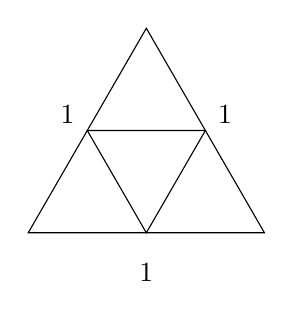
\begin{tikzpicture}[scale=1, transform shape]
					\draw (0,0) -- ++(60:3) -- ++(300:3) -- cycle;
					\draw (1.5,-0.5) node {$1$};
					\draw (0.5,1.5) node {$1$};
					\draw (2.5,1.5) node {$1$};

					\draw (1.5,0) -- ++(60:1.5) -- ++(180:1.5) -- cycle;
				\end{tikzpicture}
			\end{center}
		\end{figure}
		Los puntos son lo polluelos y los $4$ subtriángulos los hoyos.
		\[
			\boxed{n=5}
		\]
		Si se mide solo el perímetro habrían 6 segmentos y $n$ sería $6$
	\item ¿Qué número de patrones de largo $n$ binarios no tienen unos consecutivos?
		\[
			b_n
		\]
		\begin{center}
			\begin{tabular}{c|c}
				$n$ & $b_n$\\
				\hline
				$0$ & $1$\\
				$1$ & $2$\\
				$2$ & $3$\\
				$3$ & $5$\\
				$4$ & $8$\\
			\end{tabular}
		\end{center}
		\[
			b_n = b_{n-1} + b_{n-2}\\
		\]
		$Z_n$: \# de patrones binarios de largo $n$ que no tienen unos consecutivos y terminan
		en cero\\
		$U_n$: \# de patrones binarios de largo $n$ que no tienen unos consecutivos y terminan
		en uno.
		\begin{align*}
			b_n &= Z_n + U_n\\
			\\
			Z_n &= b_{n-1}\quad n \geq 1 && \text{El número de patrones anteriores más un $0$}\\
			U_n &= Z_{n-1}=b_{n-2}\quad n \geq 2 && \text{El número de $Z$'s anteriores mas un $1$}\\
			\\
			&\begin{cases}
				b_n &= b_{n-1}+b_{n-2}\\
				b_1 &= 2\\
				b_2 &= 3
			\end{cases}
		\end{align*}
	\item Tenemos banderas rojas de $1m$ de alto.
		Verdes de $2m$ de alto.
		Azules de $2m$ de alto.
		Negras de $3m$ de alto.

		¿De cuantas formas podemos ordenar banderas en un poste de $n$ metros de alto
		si el orden de las banderas importa? (Sin espacios vacios)
		\begin{center}
			\begin{tabular}{c|c|c}
				$n$ & $f_n$ & Patrones\\
				\hline
				$0$ & $1$ & $\cancel{O}$\\
				$1$ & $1$ & R\\
				$2$ & $3$ & RR,V,A\\
				$3$ & $6$ & RRR,VR,AR,RV,RA,N\\
				$4$ & $13$ & RRRR,RRV,RRA,RVR,RAR,VRR,ARR,RN,NR,AA,AV,VA,VV\\
			\end{tabular}
		\end{center}
		\begin{align*}
			\begin{cases}
				f_n &= f_{n-1}+f_{n-2}+f_{n-2}+f_{n-3}\\
				f_n &= f_{n-1}+2f_{n-2}+f_{n-3}\quad n \geq 4\\
				f_1 &= 1\\
				f_2 &= 3\\
				f_3 &= 6
			\end{cases}
		\end{align*}
\end{enumerate}

\end{document}
%}}}
